\FloatBarrier
\label{sec:mitigateNN}
Local environmental mass-density fluctuations produce so-called Newtonian noise (NN) in a gravitational-wave detector through direct gravitational coupling with its test masses. Density perturbations can be associated with seismic, sound, temperature, and humidity fields, but also be produced by moving and vibrating objects. Newtonian-noise cancellation comprises techniques where auxiliary sensors are deployed to monitor sources of density perturbations, and their data are then used to produce a NN estimate that is being subtracted from the GW detector data.

As described in Section \ref{SiteReq}, the first step of any NN mitigation strategy is to reduce environmental disturbances. For ET, this includes site selection, underground construction, and realizing a low-noise detector infrastructure. However, only if the natural environment is among the quietest in the world, and excess anthropogenic noise can be avoided, then it might be possible to achieve the ET sensitivity target without NN cancellation. Nonetheless, without a detailed understanding of the seismic field, which is hard to obtain even with an extensive site-characterization study, NN modeling uncertainties are significant. It is therefore necessary to include NN cancellation in the R\&D plans.
\begin{figure}[t!]
    \centering
    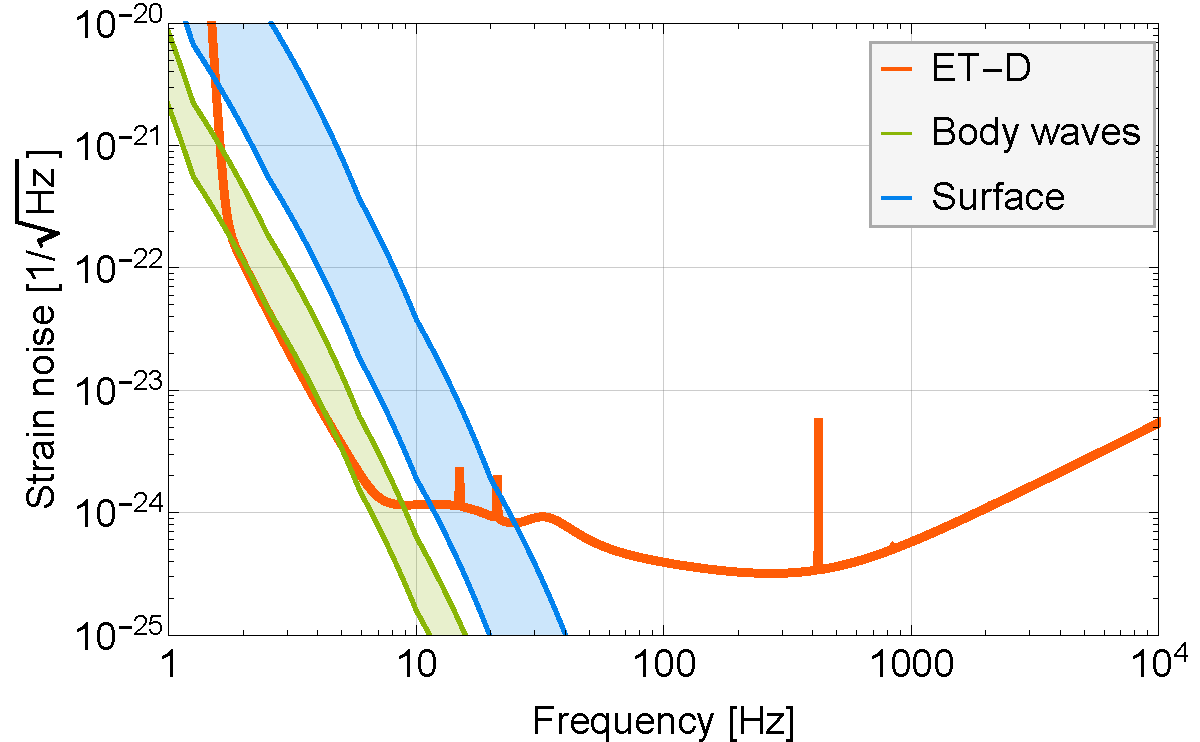
\includegraphics[width=0.49\textwidth]{SiteInfra/SiteRequirements/NewtonianNoise/NewtonianNoiseFigures/Seismic_Surf.pdf}
    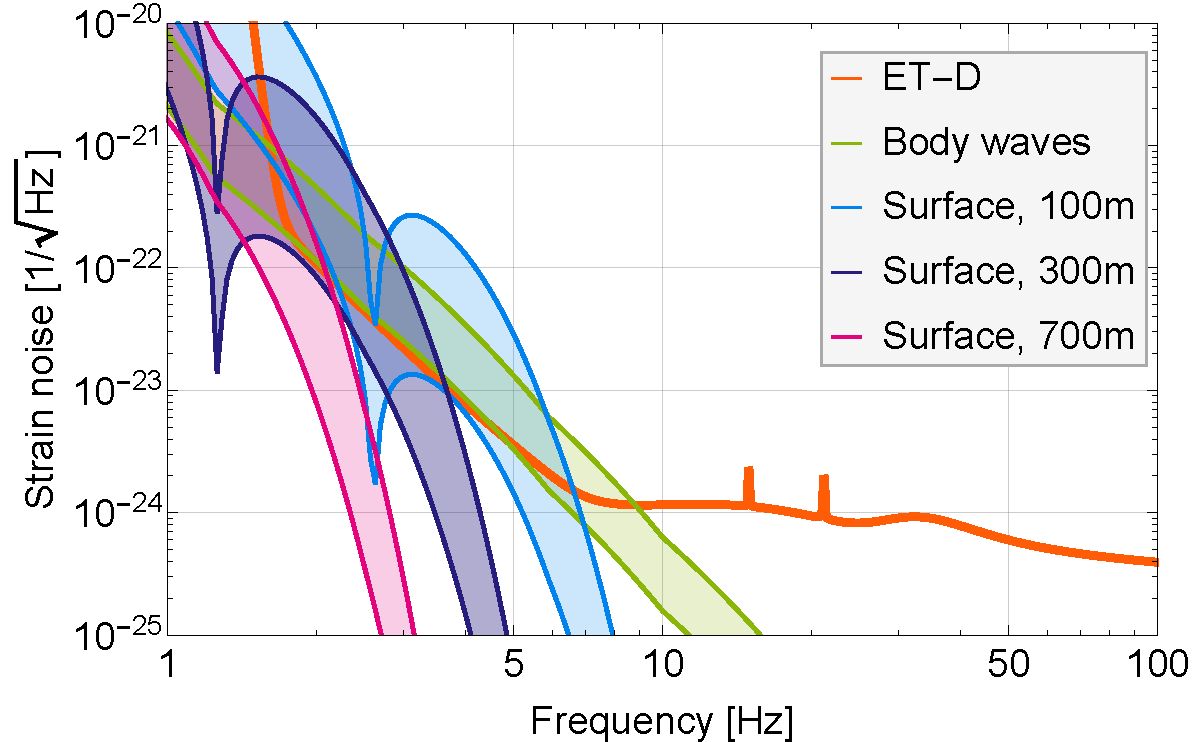
\includegraphics[width=0.49\textwidth]{SiteInfra/SiteRequirements/NewtonianNoise/NewtonianNoiseFigures/Seismic_UG.pdf}
    \caption{Estimates of seismic NN for ET. Left: ET constructed at the surface. Right: ET constructed underground. Plot from \cite{BaHa2019}.}
    \label{fig:NNestimates}
\end{figure}

As shown in Figure \ref{fig:NNestimates}, NN from surface waves will be strongly suppressed if the detector is constructed a few 100\,m underground. However, the NN from seismic body waves cannot be avoided at any depth, and it becomes a sensitivity-limiting noise contribution below 10\,Hz. Depending on the quality of the underground site, one still needs to mitigate body-wave NN by up to a factor 10. The range of body-wave NN shown in the two plots assumes that underground seismic spectra are a factor 3 to 12 above the global low-noise model \cite{Pet1993}, and an isotropic field is composed entirely of compressional waves. If it were composed entirely of shear waves, then the NN would be a factor 2 smaller. The prediction of Rayleigh NN (denoted {\it Surface} in the two plots) in underground detectors requires an assumption about the seismic surface spectrum, which is a factor 50 to 1000 above the global low-noise models in the two plots, but also an assumption about the dispersion curve. The slower (and therefore shorter) Rayleigh waves, the stronger is the suppression of associated NN with depth \cite{Har2015}. The dispersion model used for the two plots (Rayleigh wavelength plays a negligible role for NN in surface detectors) yields a Rayleigh-wave speed of 1.5\,km/s at 1\,Hz falling to 300\,m/s at 10\,Hz. There can be significant regional variations, but these values are typical. For the body-wave and Rayleigh-wave field, anisotropy can increase or decrease NN relative to the isotropic level shown in Figure \ref{fig:NNestimates}.

\subsection{Coherent noise cancellation}
\label{sub:Wiener}
The basic idea for noise cancellation is to exploit correlations between NN and data from a set of auxiliary sensors. An effective technique is to use Wiener filters \cite{Orf2007}. They are the optimal linear filters for this purpose provided that all time series are stationary, and they are effective even in the presence of non-stationary features in the data. Wiener filters can be estimated from data. It requires the calculation of correlations between all auxiliary sensors monitoring the environment, which form a correlation matrix $\mathbf C_{\rm SS}$, and between auxiliary sensors and GW detector, which form a vector $\vec C_{\rm SN}$. Since one is mostly interested in the frequency-domain representation of detector noise, correlations are expressed as cross-spectral densities depending on frequency $\omega$. The Wiener filter can then be written
\begin{eqnarray}
		\vec w(\omega)=\mathbf C_{SS}(\omega)^{-1}\cdot\vec C_{\rm SN}(\omega)
		\label{eq:Wiener}
\end{eqnarray}
This filter is applied to discrete Fourier transforms of data from auxiliary sensors, $\vec d(\omega_i)$, to produce an estimate $\hat n(\omega_i)=\vec w(\omega_i)^\dagger\cdot \vec d(\omega_i)$ of NN, which is then subtracted from the GW detector data. In average, the relative suppression of NN by a Wiener filter is given by
\begin{eqnarray}
		\epsilon(\omega)=\sqrt{1-\frac{\vec C^\dagger_{\rm SN}(\omega)\cdot \mathbf C_{\rm SS}(\omega)^{-1}\cdot\vec C_{\rm SN}(\omega)}{C_{\rm NN}(\omega)}},
		\label{eq:residual}
\end{eqnarray}
where $C_{\rm NN}(\omega)$ is the spectral density of NN in the GW detector. This expression tells us that to achieve a good subtraction efficiency, three conditions are to be met:
\begin{itemize}
\item All the sensors should be coupled as much as possible to NN. In other words, the correlation $\vec C_{\rm SN}$ between sensor outputs and GW detector must be large.
\item The correlations between sensors, described by the matrix $\mathbf C_{\rm SS}$, which also include sensor noise on its diagonal, must be small.
\end{itemize}
Designing a NN cancellation system for a GW detector that is yet to be built, only the correlations among auxiliary sensors $\mathbf C_{\rm SS}$ can be measured during a site-characterization campaign. A model is required using the correlations $\mathbf C_{\rm SS}$ to obtain $\vec C_{\rm SN}$ and $C_{\rm NN}$ \cite{CoEA2016a}.

The theory of Wiener filtering does not directly address a major challenge of NN cancellation, which is the optimal placement of auxiliary sensors. This aspect is very important for the cancellation of NN from seismic and atmospheric fields. Analyses of optimal array configurations are important since, even when lacking an accurate understanding of environmental fields, optimization results provide useful estimates of the required number of auxiliary sensors, the required sensitivity of sensors, and an approximate idea of how far from the test masses sensors need to be placed. This aspect is discussed in Section \ref{sub:optimization}.

\subsection{Site properties relevant to Newtonian-noise cancellation}
\label{sub:properties}
Since the Wiener filter is based on correlations in environmental fields, anything that influences these correlations affects NN cancellation. In the following, site properties relevant to seismic and atmospheric NN are briefly described.

\subsubsection*{Seismic fields}
\begin{itemize}
\item {\bf Seismic speed}\; Seismic correlations and correlations of seismic NN between test masses decrease with increasing distance. In frequency domain, this can be quantified in terms of a spatial correlation function $\mathcal F$ that assumes its maximal value 1 when the two seismometers or test masses are sharing the same location. As a function of the separation $L$, one finds for isotropic Rayleigh-wave fields
\begin{eqnarray}
	\mathcal{F}_{\rm NN}=J_{0}(2\pi L/\lambda)-J_{2}(2\pi L/\lambda),\quad \mathcal{F}_{\rm seis}=J_{0}(2\pi L/\lambda).
	\label{eq:geometrical}
\end{eqnarray}
As is intuitively clear, how quickly correlation decreases with increasing distance $L$ depends on the length $\lambda$ of a Rayleigh wave. The first zero of the seismic correlation is at a distance of about $0.4\lambda$. Correlations of NN between two test masses of one arm separated by several kilometers can be neglected. Due to equation (\ref{eq:residual}), seismometer arrays used for NN cancellation ideally have diameters similar to the length a Rayleigh wave. 

\item {\bf Wave polarizations}\; Seismic-wave polarizations play a major role in NN cancellation. The two main polarizations are shear and compressional waves, and Rayleigh surface waves are a so-called inhomogeneous (amplitude decreasing exponentially with depth) extension of a superposition between these two polarizations. The composition of the seismic field in terms of wave polarizations varies between sites, and depends on local geology as well as on the type and location of seismic sources. All polarizations produce NN either through compression of the medium or by displacement of surfaces and interfaces.

If only one wave polarization is present at a time, then it is almost trivial to cancel associated NN \cite{Har2015,HaVe2016}. A mix of wave polarizations can however make it very difficult to cancel a significant amount of NN \cite{HaVe2016,BaHa2019}. The issue is that correlations between seismometers and test mass decrease more quickly with distance when multiple polarizations are present, which hampers efficient noise cancellation as pointed out in Section \ref{sub:Wiener}. As a consequence, a larger number of seismometers is required to be able to be distinguish between polarizations and be susceptible to the correlations of each wave type. 

\item {\bf Seismic sources}\; The distribution and type of seismic sources both influence the composition of a seismic field. Most important to know is whether seismic sources are local or distant, and whether they are underground or at the surface. Some sources might not even fall into a clear category if it is for example a surface structure anchored to a deeper part of the ground. With respect to environmental noise, it is one of the most important tasks of a site-characterization campaign to identify as many seismic sources as possible. A NN cancellation scheme can be greatly simplified or be made significantly more effective if understanding about the seismic sources is used. Furthermore, excess noise produced by the infrastructure of the Einstein Telescope will also pose additional challenges for the design of a NN cancellation system. 

\item {\bf Local topography and geology}\; Two-point correlations of the seismic field can be affected by topography and geology. Generally, seismic-wave reflections from surfaces and interfaces cause conversions between wave polarizations. Scattering from non-planar structures can also give rise to local field components that strongly decay with distance. These local components are very similar in nature to the near-field of seismic sources. In the presence of significant geological heterogeneities or rough surface topography, it is therefore more challenging to collect all information required to design seismometer arrays for efficient NN cancellation \cite{CoHa2012}. Especially in relatively noisy environments with elevated NN where more efficient cancellation of NN might be required, site characterization should therefore assess geological properties and topography also in the context of NN cancellation.

\end{itemize}

\subsubsection*{Atmospheric fields}
Avoiding NN from the atmosphere is an important reason to construct the Einstein Telescope underground. In Section \ref{sec:envnoise}, some of the complexity of atmospheric fields and how they produce NN are described. There are serious practical challenges to design a cancellation system for atmospheric NN. 

\begin{itemize}
\item {\bf Wind noise}\; The variety of phenomena makes the monitoring of the atmosphere a challenging task. One strategy for NN cancellation would be to monitor sound, wind speed, temperature and humidity fields. Sound is typically measured with microphones. However, pressure fluctuations produced by turbulent flow in the vicinity of a microphone can mask an underlying sound signal \cite{Gre2015}. This contribution is often called wind noise. Clever sensor design, averaging pressure signals over some baseline, or constructing wind shields can prove effective \cite{Ell1972,WaHe2009,NoEA2014}. However, when it comes to an order of magnitude suppression of NN from sound, then even a small incoherent contribution to signals from wind noise can be detrimental. For this reason, entirely new approaches need to be considered. 

\item {\bf LIDAR}\; LIDAR (derived from \emph{light} and \emph{radar}) technology has been applied to investigate microscale physics in the atmospheric boundary layer. It consists of a laser beam that scatters back from the atmosphere carrying information about the presence of certain molecules, or wind speed \cite{CLN2004}, temperature \cite{Beh2005}, etc. Volumetric observations can be performed to characterize the evolution of entire fields. It is conceivable that a LIDAR system can be developed in the foreseeable future to cancel at least modest amounts of wind-driven NN associated with temperature and humidity fields. However, atmospheric density perturbations due to sound are orders of magnitude weaker in the ET observation band, which makes it extremely challenging to develop a LIDAR to monitor sound fields.

\item {\bf Cavity atmosphere}\; Potentially significant NN contributions can come from the sound field inside the cavities hosting the test masses of the Einstein Telescope \cite{FiEA2018}. Due to the absence of fast air currents, wind noise in microphones located inside the cavity will be strongly reduced, and high-precision sound monitoring would be possible. At the same time, absence of fast air currents also means that all forms of cavity atmospheric NN driven by wind, i.e., associated with temperature and humidity fields, will be negligible. This means that cancellation from cavity atmospheric NN should be possible using an array of microphones.
\end{itemize}

\subsection{Optimized sensor arrays for seismic NN cancellation}
\label{sub:optimization}

Another important point to understand is how the subtraction procedure improves with the number of sensors, and how much it is sensitive to a non optimal placement of the sensors. This is important because in a practical implementation, the possibility of optimizing the placement of underground sensors will be limited. 

Optimized seismometer arrays were initially studied for the cancellation of NN from Rayleigh waves \cite{DHA2012,Har2015,CoEA2016a}, and more recently from body waves \cite{BaHa2019}. Array optimization was based on simplified models of the seismic field in all these publications, which means that the calculated array configurations are not of direct use for NN cancellation in real environments. However, the total number of seismometers and the seismometer sensitivity required to achieve a certain cancellation performance are less dependent on the model of the seismic field \cite{CoEA2016a}. 

Accordingly, Fig.~\ref{fig:residualN} gives an estimate of the required number of seismometers to cancel a certain amount of body-wave NN provided that they assume their optimal positions. 
\begin{figure}[t!]
	\begin{center} 
		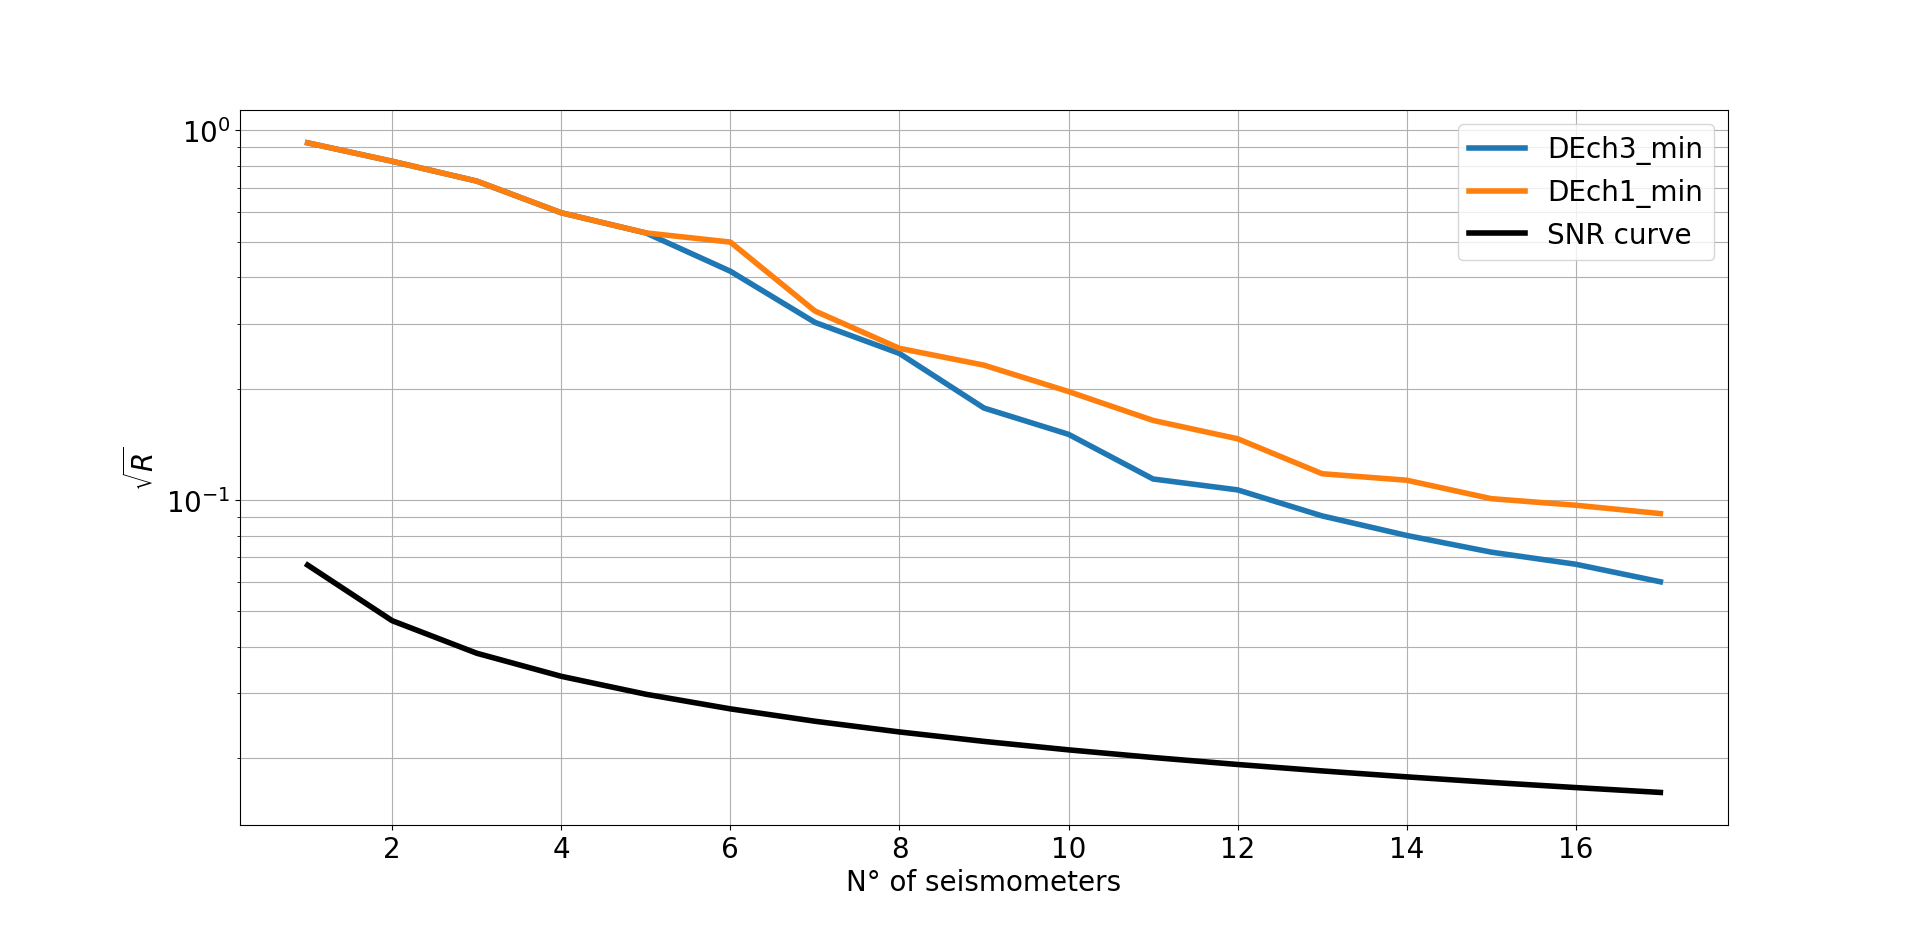
\includegraphics[width=0.7\textwidth]{SiteInfra/SiteRequirements/NewtonianNoise/NewtonianNoiseFigures/SNR_ch3.png}
		\caption{Suppression of body-wave NN as a function of number of seismometers with optimal placement. The seismometers measure seismic signals with an SNR of 15. The black curve shows the lowest possible residual determined by the seismometer SNR without considering properties of the seismic field. Plot from \cite{BaHa2019}.} 
		 \label{fig:residualN} 
	\end{center}
\end{figure}
About 15 seismometers are required to achieve a factor 10 suppression. It should be emphasized that this result depends to some extent on the relative contributions of compressional waves and shear waves to the seismic field. For these results, it is assumed that compressional waves constitute 30\% of the seismic power-spectral density. Less seismometers are required if one polarization greatly dominates over the other. These instruments need to be deployed in boreholes, and the number 15 is per test mass. 

In this context, one can now address the question how accurately the seismometers need to be placed with respect to their optimal locations. While direction and vertical drilling technology has become increasingly accurate \cite{MCZ2016}, significant deviations from optimal drilling are to be expected, which results in sub-optimal seismometer placements. Figure \ref{fig:errorNN} shows the residuals that can be achieved with sub-optimal seismometer placement. 
\begin{figure}[t!]
	\begin{center} 
		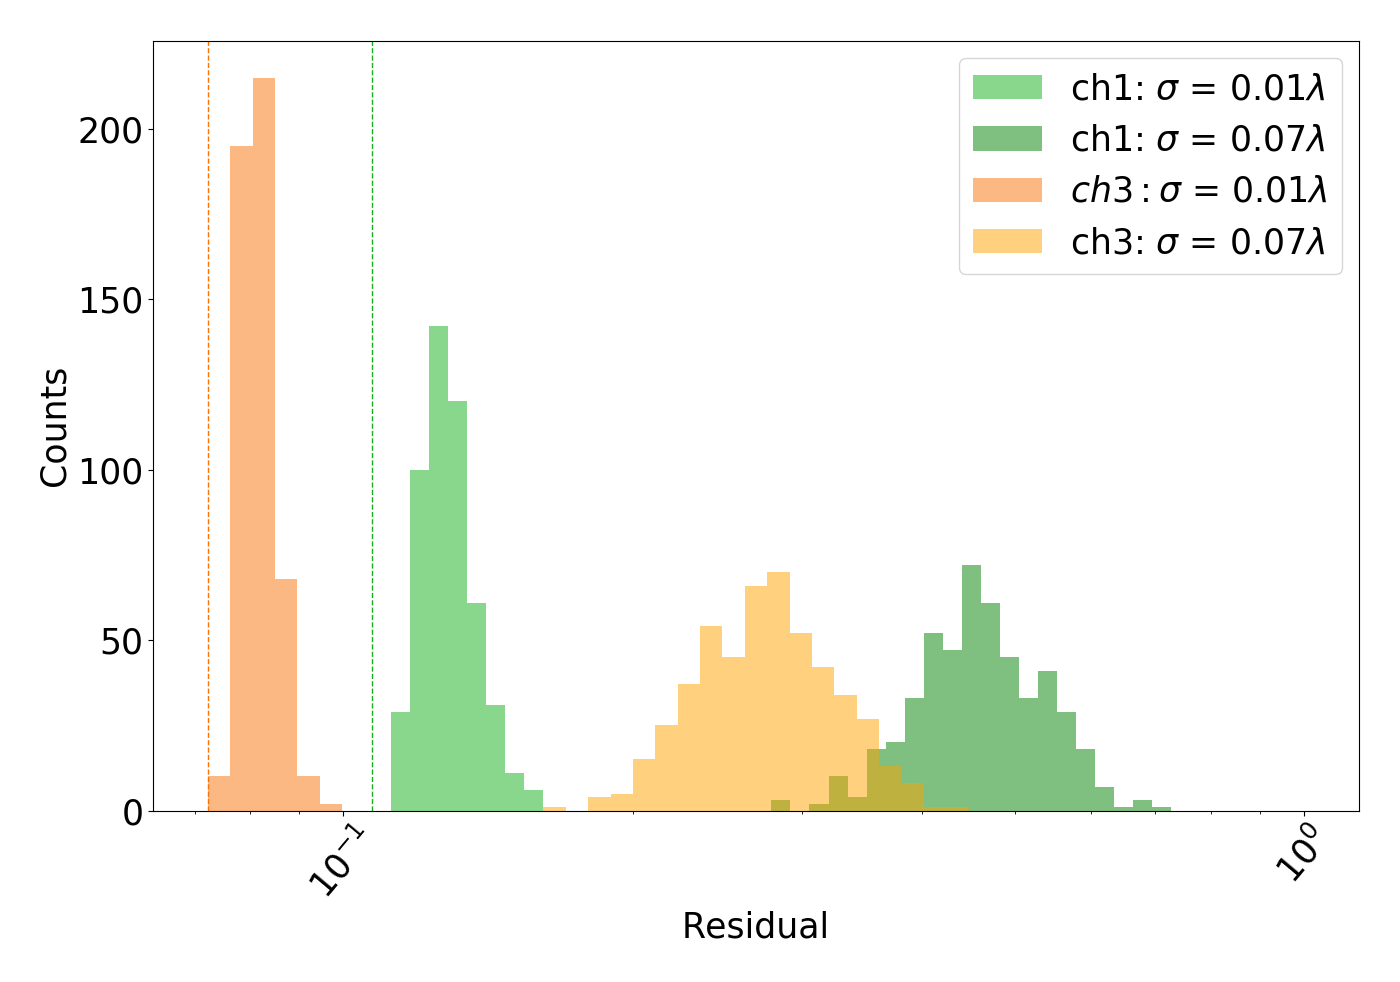
\includegraphics[width=0.7\textwidth]{SiteInfra/SiteRequirements/NewtonianNoise/NewtonianNoiseFigures/errorbody.png} 
		\caption{Suppression of NN from body waves with 15 single-axis (ch1) and three-axis (ch3) seismometers. Sensor locations of 500 arrays for each histogram are derived from the optimal array by adding random numbers to all optimal coordinates drawn from Gaussian distributions of width $\sigma$. Vertical lines mark the residual of the optimal arrays. Plot from \cite{BaHa2019}.} 
		 \label{fig:errorNN} 
	\end{center}
\end{figure}
To produce this plot, seismometer coordinates were shifted by a random number drawn from a Gaussian distribution of width $\sigma$ specified in the legend relative to the length $\lambda$ of compression waves. Assuming a compressional-wave speed of 4\,km/s, $\sigma=0.07\lambda=28\,$m at 10\,Hz. The corresponding arrays with three-axis sensors (ch3) still achieve a body-wave NN suppression by a factor 3 and better. For boreholes of a few 100\,m, and drill deviation of less than 1 degree, such sensor-placement accuracy is achievable. 

The remaining challenge is to have sufficient observations of the seismic field to be able to accurately calculate the optimal array configurations. In fact, incomplete knowledge of seismic correlations will likely lead to the dominant error in the seismometer placements. This error needs to be minimized by studying in detail the seismic field at the site of the Einstein Telescope also using borehole seismometer installations.
